\noindent \textred{3.} 
A mathematical game (or puzzle) consists of three rods and a number of disks of various diameters, which can slide onto any rod. The puzzle begins with $\textbf{n}$ disks stacked on a \textbf{start} rod in order of decreasing size, the smallest at the top, thus approximating a conical shape. The objective of the puzzle is to move the entire stack to the \textbf{end} rod, obeying the following rules:
\begin{enumerate}
    \item[i] Only one disk may be moved at a time;
    \item[ii] Each move consists of taking the top disk from one of the rods and placing it on top of another rod or on an empty rod;
    \item[iii] No disk may be placed on top of a disk that is smaller than it.
\end{enumerate}
\begin{figure}[!h]
    \centering
    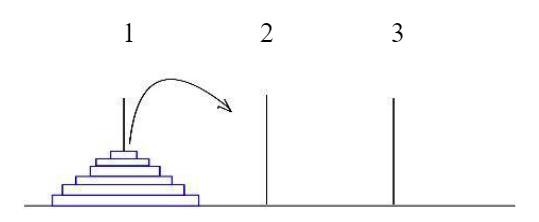
\includegraphics[width=0.4\linewidth]{HWs/HW3/HW03_03.jpg}
    % \label{fig:HW02_01_tree}
\end{figure}
Please design a MOVE(n, start, end) function to illustrate the minimum number of steps of moving n disks from start rod to the end rod. \\
You \textbf{MUST} use the following functions and format, otherwise you will not get points of part (a) and (b): 
\begin{minted}{python}
def PRINT(origin, destination):
    print("Move the top disk from rod", origin, "to rod", destination)

def MOVE(n, start, end): # TODO: you need to design this function
    pass
\end{minted}
For example, the output of MOVE(2, 1, 3) should be: \\
Move the top disk \textbf{from} rod 1 to rod 2 \\
Move the top disk \textbf{from} rod 1 to rod 3 \\
Move the top disk \textbf{from} rod 2 to rod 3 
\begin{enumerate}
    \item[(a)] Give the output of MOVE(4, 1, 3). \\
    \textblue{
        Move the top disk \textbf{from} rod 1 to rod 2 \\
        Move the top disk \textbf{from} rod 1 to rod 3 \\
        Move the top disk \textbf{from} rod 2 to rod 3 \\
        Move the top disk \textbf{from} rod 1 to rod 2 \\
        Move the top disk \textbf{from} rod 3 to rod 1 \\
        Move the top disk \textbf{from} rod 3 to rod 2 \\
        Move the top disk \textbf{from} rod 1 to rod 2 \\
        Move the top disk \textbf{from} rod 1 to rod 3 \\
        Move the top disk \textbf{from} rod 2 to rod 3 \\
        Move the top disk \textbf{from} rod 2 to rod 1 \\
        Move the top disk \textbf{from} rod 3 to rod 1 \\
        Move the top disk \textbf{from} rod 2 to rod 3 \\
        Move the top disk \textbf{from} rod 1 to rod 2 \\
        Move the top disk \textbf{from} rod 1 to rod 3 \\
        Move the top disk \textbf{from} rod 2 to rod 3 \\
    }
    \item[(b)] Fill in the function MOVE(n, start, end) shown above. You can use Python, C/C++ or pseudo-code form, as you want.

% \begin{figure}[h]
% \centering
% \begin{minipage}[c]{0.87\linewidth}
\begin{minted}{python}
def MOVE(n, start, end): # Python code
    if n == 1:
        PRINT(start, end)
    else:
        temp_rod = 6 - start - end
        MOVE(n-1, start, temp_rod)
        MOVE(1, start, end)
        MOVE(n-1, temp_rod, end)
\end{minted}
% \end{minipage}
% \end{figure}
    \item[(c)] What’s the minimum number of moves of MOVE(5, 1, 3), and MOVE(n, 1, 3)? \\
    \textblue{
    Minimum moves of MOVE(5, 1, 3): \underline{31} \\
    Minimum moves of MOVE(n, 1, 3): \underline{$2^n - 1$} \\
    }
\end{enumerate}

